\documentclass[12pt,fleqn]{article}
\setlength{\parindent}{0pt}
\usepackage{graphicx}
\usepackage{listings}
\usepackage[latin5]{inputenc}
\setlength{\parskip}{8pt}
\setlength{\parsep}{0pt}
\setlength{\headsep}{0pt}
\setlength{\topskip}{0pt}
\setlength{\topmargin}{0pt}
\setlength{\topsep}{0pt}
\setlength{\partopsep}{0pt}
\setlength{\mathindent}{0cm}

\begin{document}
MIT OCW Cok Degiskenli Calculus - Ders 8

Iki degiskenli bir fonksiyonu grafiklemek (plot) icin 

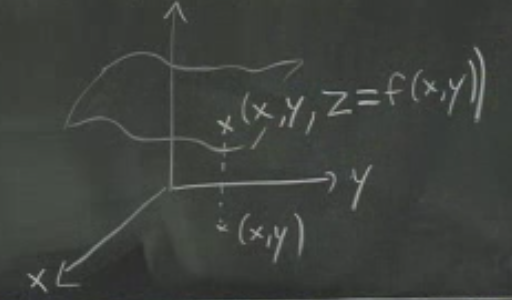
\includegraphics[height=4cm]{8_1.png}

$x,y$ degerlerine tekabul eden $f(x,y)$'yi, z ekseni uzerindeki yukseklik
olarak kabul ederiz, ve oraya bir nokta koyariz. Tum $x,y$'ler icin bu
yapilirsa bir yuzey ortaya cikar. Dikkat 3 boyutlu bir sekil gorulecektir,
fakat ici dolu degildir, fonksiyon sadece yuzeydedir. 

Ornek

\[ f(x,y) = -y \]

2 degiskenli de olsa illa her iki degisken fonksiyonda kullanilmali diye
bir sart yok. Bu formul bir duzlem tanimlar. 

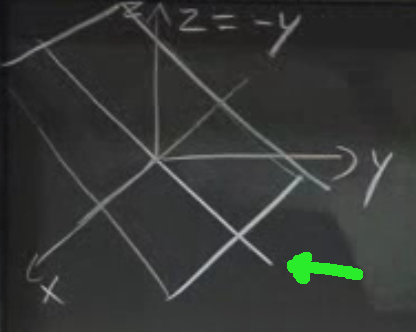
\includegraphics[height=4cm]{8_2.png}

Hoca cizmek icin once yesil okun gosterdigi cizgiden basladi, ki bu cizgi
$z=-y$, -1 egimi olan bir cizgi. $x$ tanimli olmadigina gore bu cizgi her
$x$ icin gecerli olmali, ve ustteki duzlem ortaya cikiyor. x-ekseni bu
duzlemin icinden geciyor. 

Ornek 

\[ f(x,y) = 1-x^2-y^2 \]

Grafigi anlamak icin $yz$ duzleminde neler oluyor onu anlamaya
ugrasalim. Sadece $yz$ duzlemine bakmak demek, $x=0$ kabul etmek demektir,
o zaman geri kalanlar 

\[ z = 1-y^2 \]

bir parabolu tanimlar. 

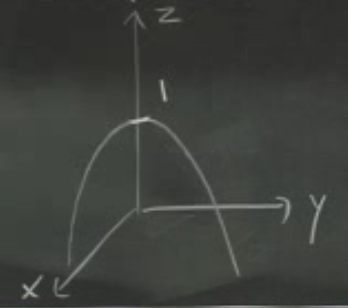
\includegraphics[height=4cm]{8_3.png}






\end{document}
